\chapter{Eksperymenty\label{chap:eksperymenty}}

\section{Parametry wejściowe oraz maszyna testowa}

\section{Wyniki eksperymentów}

\subsection{Wyniki pomiarów poszczególnych implementacji algorytmów}

\subsubsection{Wyniki dla minsup = 0.2, minconf = 0.1}

\begin{figure}[ht]
\centering
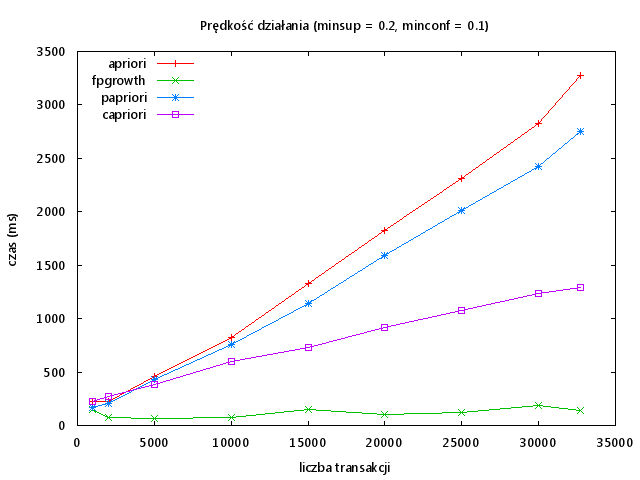
\includegraphics[width=1.1\textwidth]{figures/06/02_01.png}
\caption{Prędkość działania algorytmów}
\end{figure}

\begin{figure}[ht]
\centering
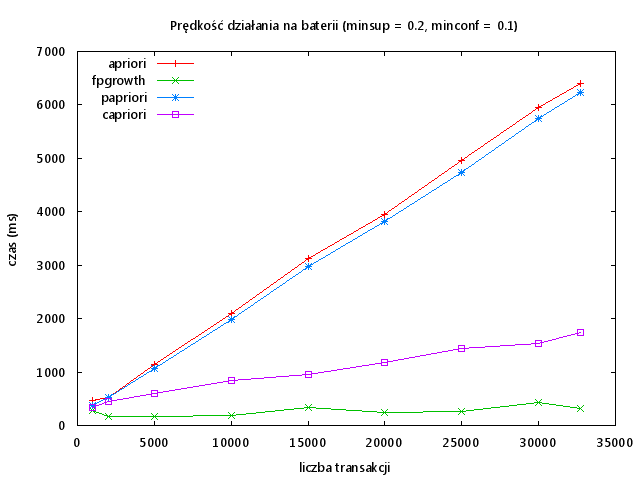
\includegraphics[width=1.1\textwidth]{figures/06/02_01_bat.png}
\caption{Prędkość działania algorytmów na baterii laptopa}
\end{figure}

\begin{figure}[ht]
\centering
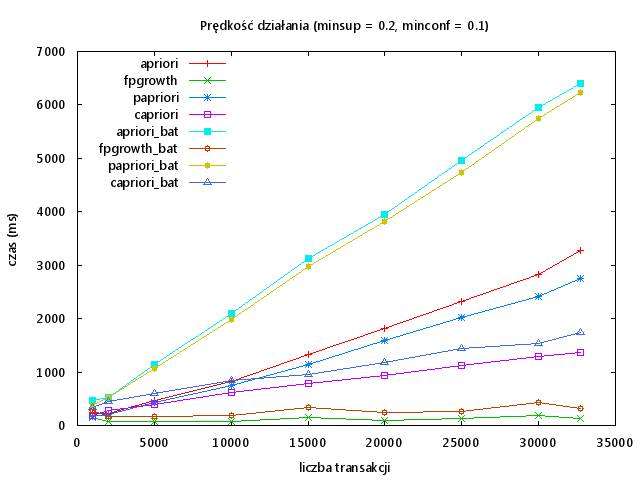
\includegraphics[width=1.1\textwidth]{figures/06/02_01_all.png}
\caption{Prędkość działania algorytmów w dwóch środowiskach uruchomieniowych}
\end{figure}

\subsubsection{Wyniki dla minsup = 0.2, minconf = 0.4}


\begin{figure}[ht]
\centering
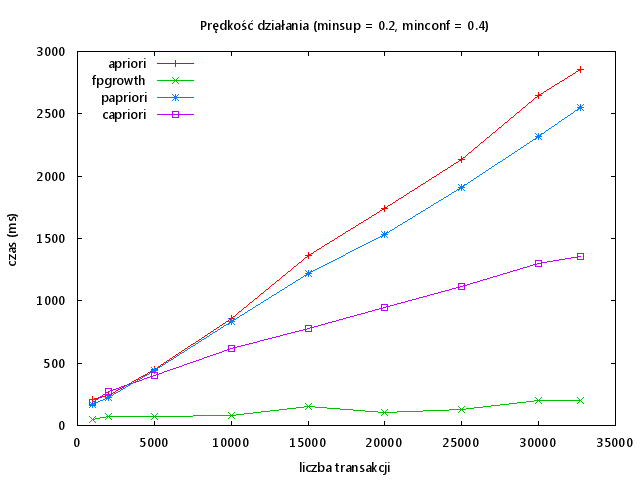
\includegraphics[width=1.1\textwidth]{figures/06/02_04.png}
\caption{Prędkość działania algorytmów}
\end{figure}

\begin{figure}[ht]
\centering
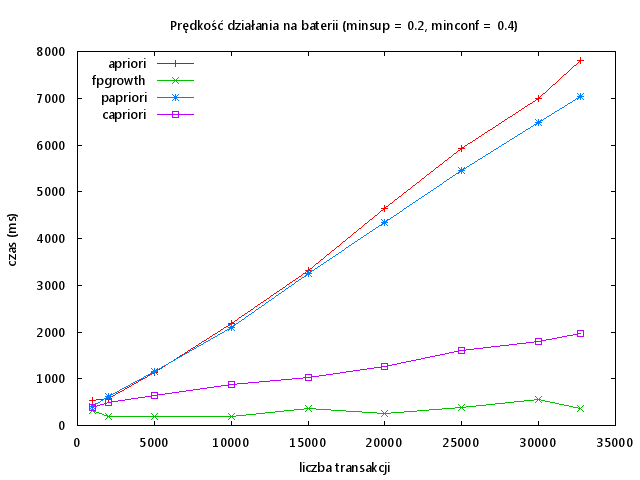
\includegraphics[width=1.1\textwidth]{figures/06/02_04_bat.png}
\caption{Prędkość działania algorytmów na baterii laptopa}
\end{figure}

\subsubsection{Wyniki dla minsup = 0.05, minconf = 0.1}

\begin{figure}[ht]
\centering
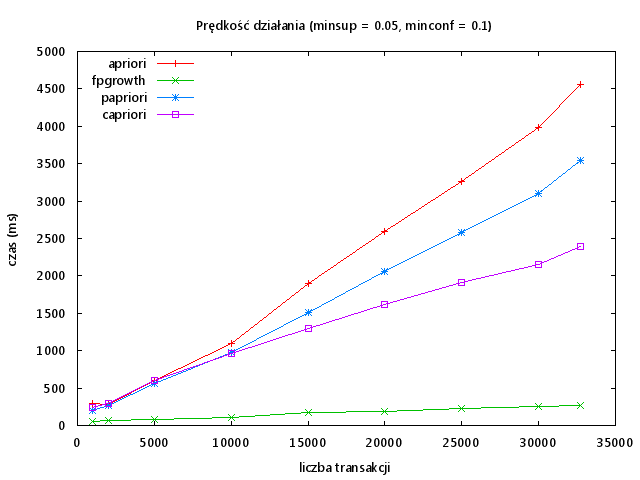
\includegraphics[width=1.1\textwidth]{figures/06/005_01.png}
\caption{Prędkość działania algorytmów}
\end{figure}

\begin{figure}[ht]
\centering
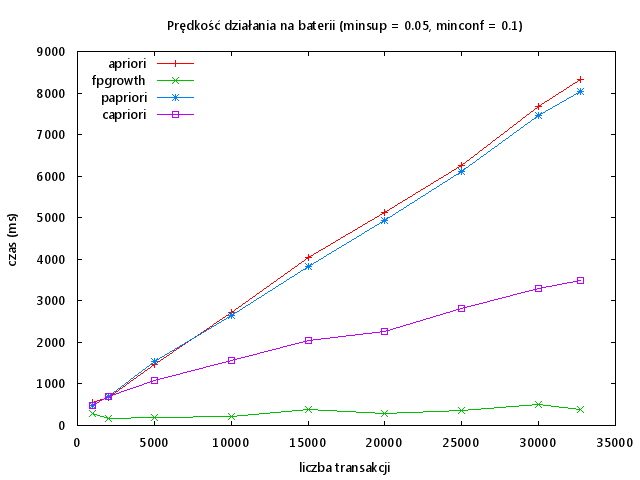
\includegraphics[width=1.1\textwidth]{figures/06/005_01_bat.png}
\caption{Prędkość działania algorytmów na baterii laptopa}
\end{figure}

\subsubsection{Wyniki dla minsup = 0.05, minconf = 0.4}

\begin{figure}[ht]
\centering
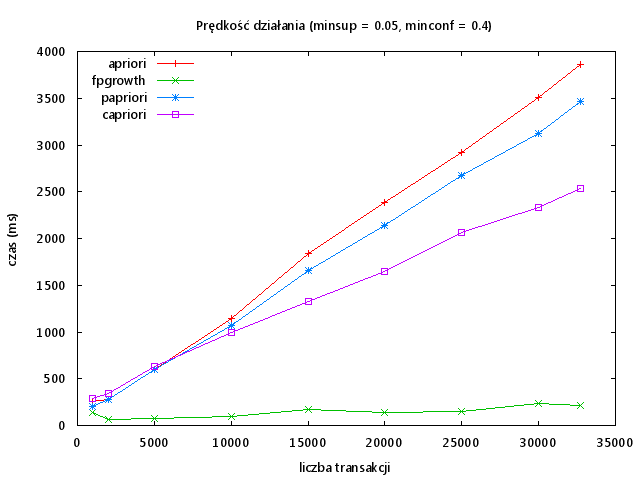
\includegraphics[width=1.1\textwidth]{figures/06/005_04.png}
\caption{Prędkość działania algorytmów}
\end{figure}

\begin{figure}[ht]
\centering
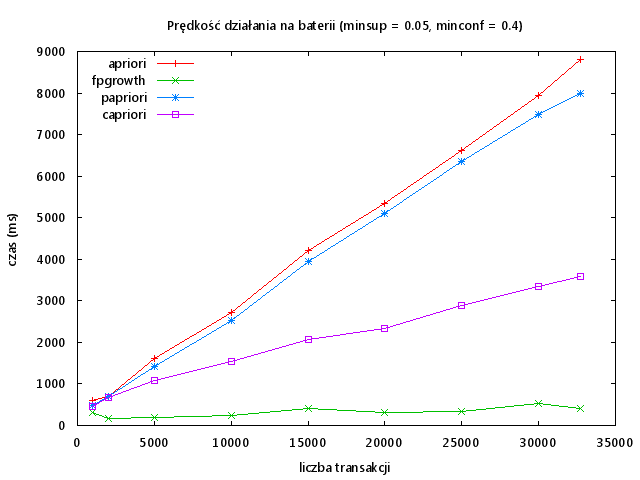
\includegraphics[width=1.1\textwidth]{figures/06/005_04_bat.png}
\caption{Prędkość działania algorytmów na baterii laptopa}
\end{figure}

\subsection{Wyniki pomiarów dla algorytmu CudaApriori}


\begin{figure}[ht]
\centering
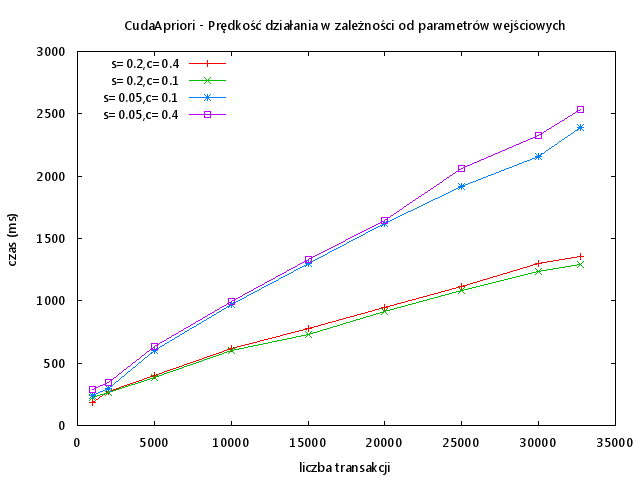
\includegraphics[width=1.1\textwidth]{figures/06/capriori.png}
\caption{Prędkość działania algorytmu CudaApriori w zależności od parametrów wejściowych}
\end{figure}

\begin{figure}[ht]
\centering
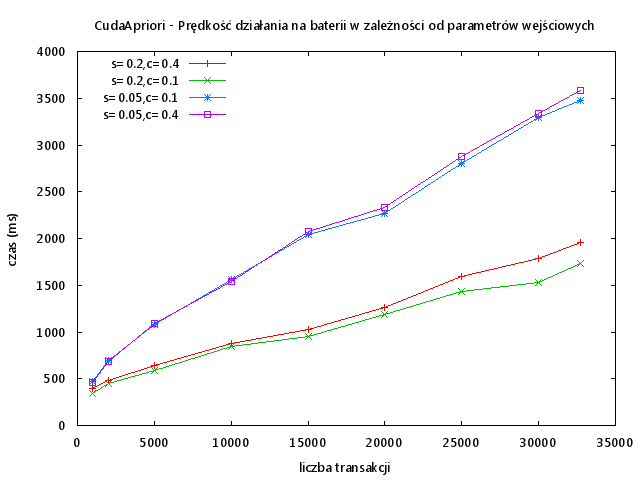
\includegraphics[width=1.1\textwidth]{figures/06/capriori_bat.png}
\caption{Prędkość działania algorytmu CudaApriori na baterii laptopa w zależności od parametrów wejściowych}
\end{figure}

\section{Podsumowanie eksperymentów i wnioski}